
%---------------------导言区---------------------------%
\documentclass[12pt,a4paper,UTF8]{ctexart}
	%10pt:正文字体为12pt,缺省为10pt;各层级字体大小会根据正文字体自动调整
	%a4paper:纸张大小a4;
	%UTF8:中文要求
\usepackage{geometry}%用于设置上下左右页边距
	\geometry{left=2.5cm,right=2.5cm,top=3.2cm,bottom=2.8cm}
\usepackage{xeCJK,amsmath,paralist,enumerate,booktabs,multirow,graphicx,subfig,setspace,listings,lastpage,hyperref,setspace}
	%xeCJK:中文字体(如楷体,作者和机构需要用到)的设置
	%amsmath:数学公式
	%paralist,enumerate:自定义项目符号
	%booktabs:三线图,论文常用的表格风格
	%multirow:复杂表格
	%graphicx,float: 插入图片
	%subfig:并排排版图片、竖向排版图片
	%setspace:设置行间距等功能
	\setlength{\parindent}{2em}%正文首行缩进两个汉字
	%listings:用于排版各种代码;比如matlab的代码
	\lstset{language=Matlab}%matlab代码
	%lastpage:获取总页数;
	%hyperref:超链接,和lastpage搭配.
\usepackage{fancyhdr}
	%fancyhdr:一个很强大的宏包,用于自定义设计页面风格并命名以供调用。
	\pagestyle{fancy}
	\rhead{实验C3.3 基于光纤光谱仪的吸收光谱实验}
	\lhead{基础物理实验\uppercase\expandafter{\romannumeral2}会议摘要}
	\cfoot{Page \thepage/\pageref{LastPage}}  %当前页\总页数
		%分别是右页眉、左页眉、中页脚、右页脚
	\renewcommand{\headrulewidth}{0.4pt}
	\renewcommand{\theenumi}{(\arabic{enumi})}

% \setCJKmainfont{FZShuSong-Z01S}[ItalicFont=FZKai-Z03S, BoldFont=FZHei-B01S]
%中文字体设置:使用开源字体方正书宋,方正楷体和方正黑体



%%%%%%%%%%%%%%%%%%%%%%%%%%%%%%%%%%%%%%%%%%%%%%%%%%%%%%%%%%
%%%%%%%%%%%%%%%%%%%%%%%%%正文开始%%%%%%%%%%%%%%%%%%%%%%%%%%
%%%%%%%%%%%%%%%%%%%%%%%%%%%%%%%%%%%%%%%%%%%%%%%%%%%%%%%%%%

\begin{document}

%%begin-------------------标题与信息-----------------------%%

%%标题
\begin{center}
\LARGE\textbf{实验C3.3 基于光纤光谱仪的吸收光谱实验}
\end{center}

%%信息
\begin{doublespacing}
	%doublespacing:手动两倍行距
	\centering
	\begin{tabular}{lr}
	& \\
	{\CJKfontspec{方正楷体简体} 学院:中山医学院} & {\CJKfontspec{方正楷体简体} 年级、专业:2020级临床医学(长学制)} \\
	{\CJKfontspec{方正楷体简体} 实验人姓名、学号:莫润冰~20980131} & {\CJKfontspec{方正楷体简体}合作者姓名、学号:黄健祥~20980118}\\
	\end{tabular}
\end{doublespacing}

%%end-------------------标题与信息-----------------------%%
\doublespacing
	\vspace{4em}
	%vspace:调整垂直空白,可以自己调整;缩小abstract和center(以及maketitle)的间距
	%\noindent %备用:摘要无缩进
	{\bf 摘{} 要:}
	{\zihao{-4} 本实验利用USB2000+型光纤光谱仪测量不同浓度红墨水溶液的吸收光谱,使用“BiaoQi Spesuite”软件实时测量吸收光谱,探究可见光波段红墨水吸收光谱的规律特征。同时,将吸收峰处的吸光度与红墨水浓度线性拟合,从而验证比尔定律。}
	\par%空的新行的高度。
	\textbf{关键词}:光纤光谱仪; 吸收光谱 ;线性拟合 ;比尔定律
	\vspace{3em}

	{\bf Abstract:}
	{In this experiment, USB2000+ optical fiber spectrometer was used to measure the absorption spectrum of red ink solutions with different concentrations, and "BiaoQi Spesuite" software was used to measure the absorption spectrum in real time to explore the law and characteristics of red ink absorption spectrum in visible band.Afterwards, the absorbance at the absorption peak is fitted linearly with the concentration of red ink to verify Beer's law.}
	\par%空的新行的高度。
	\textbf{Key words}:Optical fiber spectromete, Absorption spectrum, Linear fitting, Beer's law
\footnotetext[1]{{Supported and taught by Han Shen, School of Physics, Sun Yat-sen University}}
\footnotetext[2]{{Corresponding author. E-mail:\url{morb@mail2.sysu.edu.cn}}}


\newpage
\subsection*{【数据处理】}

\begin{figure}[htbp]
	\centering
	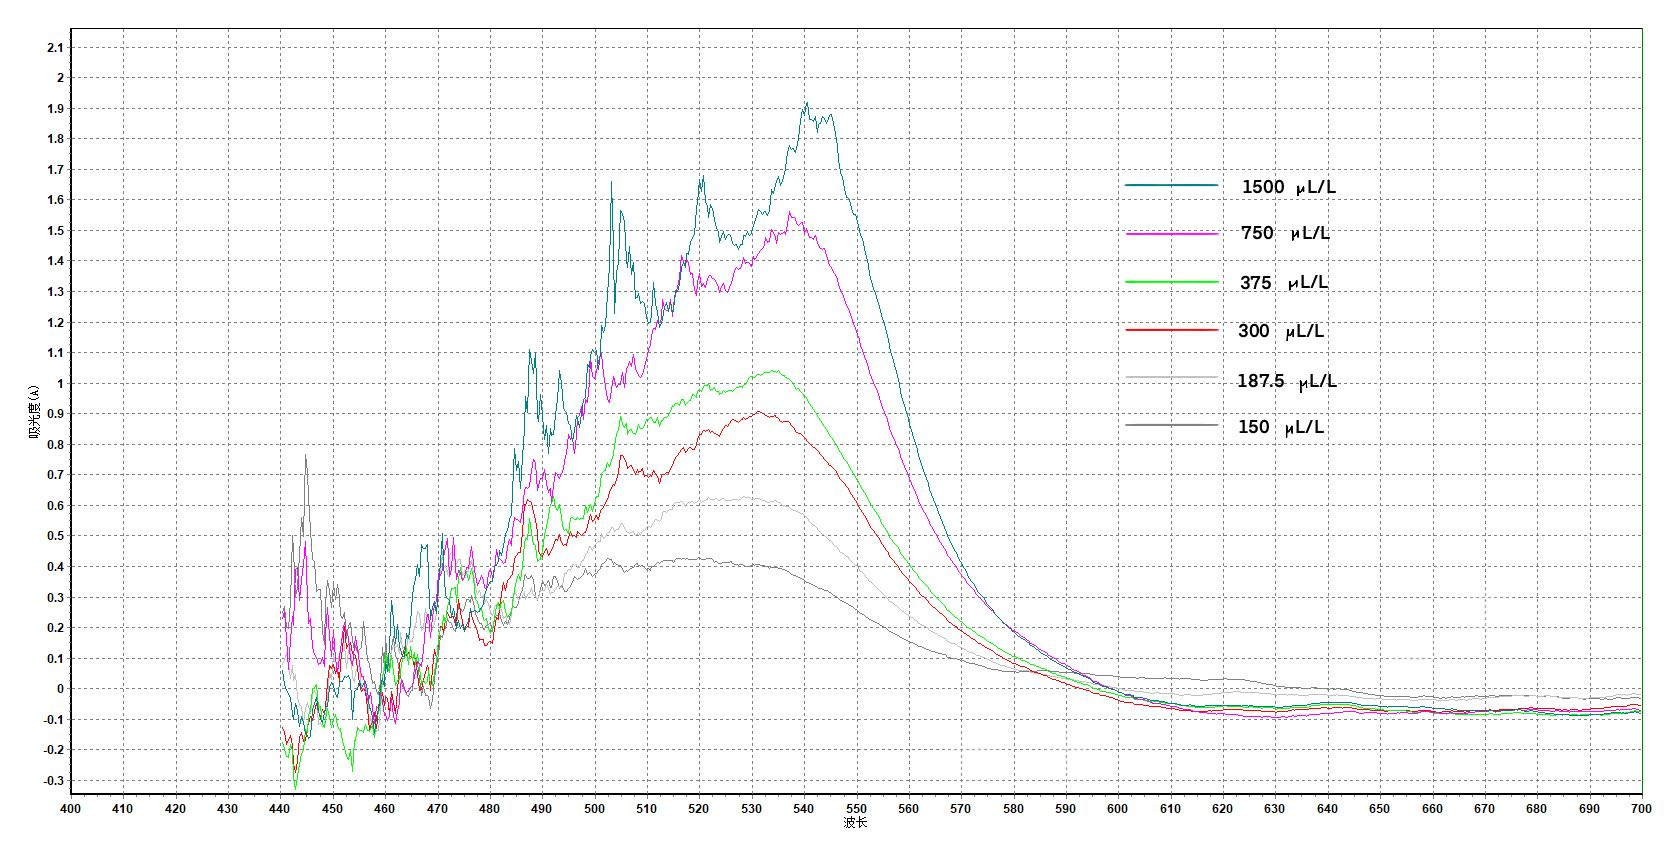
\includegraphics[width=\textwidth]{img//吸收光谱.jpg}
	\caption{不同浓度红墨水的吸收光谱}
	\label{fig:1}
\end{figure}

由\ref{fig:1}可以看出红墨水吸收峰大致在波长510nm处。


\begin{table}[htbp]
	\caption{实验数据}
	\centering
    \begin{tabular}{|c|c|c|c|c|c|c|}
	\hline
    浓度n $\mu L/L $   & 150 & 187.5 & 300 & 375 & 750 & 1500 \\
	\hline
    吸收峰波长$\lambda /nm$ & 519.973 & 528.744 & 530.845 & 534.693 & 537.140 & 540.631 \\
	\hline
    吸光度 & 0.425 & 0.625 & 0.905 & 1.036 & 1.560 & 1.919 \\
	\hline
	\end{tabular}%
	\label{tab:data}%
\end{table}%
将上述数据进行线性拟合,拟合直线如\ref{fig:2}所示,其拟合直线方程为:

\begin{equation*}
	y=0.001034x+0.516314
\end{equation*}

其中皮尔森相关系数R=0.9527492,t值为6.2731,p值为0.003296.
上述数据表示线性拟合是准确的。因此本实验很好地验证了比尔定律中溶液吸收系数与浓度成正比的关系。


\begin{figure}[htbp]
	\centering
	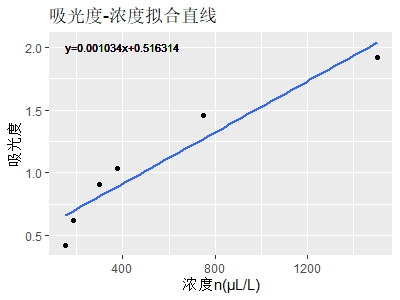
\includegraphics[width=0.8\textwidth]{img//Reg.jpeg}
	\caption{吸光度-浓度拟合曲线}
	\label{fig:2}
\end{figure}

\newpage
\subsubsection*{误差分析}
1.扫描步长比较长,故无法准确捕捉峰值的位置

2.取峰值时峰值附近数值接近,峰值模糊

3.外界光源对实验有影响,无法忽略

4.放样池外部污染,影响光谱测定

\subsection*{【思考题】}
\subsubsection*{1.根据红墨水吸收峰波长,如何选择光源?理由是什么?}
由实验测量可知,红墨水吸收峰大致在510nm处,故光源的光谱区应该覆盖这个范围,最好是以这个波长范围为中心,这样可以减小在验证比尔定律过程中的一些误差。
同时光源应具备连续的发射光谱,而且我们要选择能稳定发光的光源,以便于后续对不同浓度的吸光度的比较。溴钨灯是连续谱且其发射光谱主要集中在350-890nm,为红外区和可见光区,因此可以作为测定红墨水吸收峰实验的光源。

\subsubsection*{2. 发射光谱和吸收光谱的测量中,光路的设置上有什么异同?}
答:发射光谱和吸收光谱光路设置基本相似,但是吸收光谱在光线进入光路之前设置了溶液吸收池,以测量溶液的吸收度。

\subsubsection*{3. 光栅光谱仪和光纤光谱仪各有什么优缺点?试举若干只能采用一种光谱仪进行测量的例子。}
光纤光谱仪通常采用光纤作为信号耦合器件,将被测光耦合到光谱仪中进行光谱分析。
其优点在于,光纤的耦合非常容易,所以可以很方便地搭建起由光源、采样附件和光纤光谱仪组成的模块化测量系统,方便实验者灵活地搭建光谱采集系统。
光栅光谱仪是使光通过光栅单色仪的光栅后发生色散并将光栅单色仪发出的光线记录下来的仪器。
其优点是,适用的波长范围广,具有较大的色散率和分辨率。荧光测量可用光纤光谱仪,检测有机物官能团用光栅光谱仪。

\subsubsection*{附录}
\begin{figure}[htbp]
	\centering
	\includegraphics[width=\textwidth]{img//Ref.jpg}
\end{figure}



\end{document}
